\documentclass[11pt]{article}
\usepackage[margin=1in]{geometry}
\usepackage{amsmath, amssymb}
\usepackage{graphicx}
\usepackage{tikz}
\usepackage{physics}
\usepackage{titlesec}
\usepackage{bm}

\titleformat{\section}{\normalfont\Large\bfseries}{\thesection}{1em}{}

\title{\textbf{Deriving the Wheel Velocity Mapping for Omni-directional Drive Systems}}
\author{Physics Oracle – PulsR}
\date{}

\begin{document}

\maketitle

\section{Introduction}

In mobile robotics, a fundamental problem is determining the required angular velocities of individual wheels to achieve a desired body motion. This is especially vital for robots with holonomic or omni-directional drive systems, where multiple wheels interact in complex ways. We derive a general formula to relate the angular velocity of a wheel to the robot's translational and rotational motion.

\section{Body Velocity Representation}

Let the robot's body velocity in its local frame be represented by the vector:
\[
\mathbf{v}_b = 
\begin{bmatrix}
v_x \\ v_y \\ \omega
\end{bmatrix}
\]
where:
\begin{itemize}
    \item \(v_x\): forward velocity in the robot's local x-direction (m/s),
    \item \(v_y\): lateral velocity in the y-direction (m/s),
    \item \(\omega\): angular velocity (rad/s).
\end{itemize}

\section{Wheel Kinematics: Linear to Angular Mapping}

Each wheel is located at position \((x_i, y_i)\) and oriented at an angle \(\theta_i\) relative to the robot frame. It can only respond to the component of the velocity aligned with its rolling direction.

The translational velocity at the wheel due to rotation about the robot center is:
\[
\mathbf{v}_{\text{rot}} = \omega 
\begin{bmatrix}
 -y_i \\
 x_i
\end{bmatrix}
\]

Thus, the total velocity at the wheel is:
\[
\mathbf{v}_{\text{wheel}} = 
\begin{bmatrix}
v_x \\
v_y
\end{bmatrix}
+
\omega
\begin{bmatrix}
 -y_i \\
 x_i
\end{bmatrix}
\]

\section{Projection Onto Wheel Rolling Direction}

Let \( \hat{t}_i = \begin{bmatrix} \cos\theta_i & \sin\theta_i \end{bmatrix} \) be the unit vector in the rolling direction of wheel \( i \). The effective linear velocity that the wheel must match is the projection:

\[
v_{\text{eff}, i} = 
\hat{t}_i^T \cdot \mathbf{v}_{\text{wheel}}
\]

Substituting:

\begin{align*}
v_{\text{eff}, i} &= \begin{bmatrix}
\cos\theta_i & \sin\theta_i
\end{bmatrix}
\left(
\begin{bmatrix}
v_x \\
v_y
\end{bmatrix}
+
\omega
\begin{bmatrix}
-y_i \\
x_i
\end{bmatrix}
\right) \\
&= \cos\theta_i v_x + \sin\theta_i v_y + \omega(-y_i\cos\theta_i + x_i\sin\theta_i)
\end{align*}

Now we rewrite this as a dot product:
\[
v_{\text{eff}, i} = 
\begin{bmatrix}
\cos\theta_i &
\sin\theta_i &
(-y_i\cos\theta_i + x_i\sin\theta_i)
\end{bmatrix}
\cdot
\begin{bmatrix}
v_x \\
v_y \\
\omega
\end{bmatrix}
\]

\section{Final Mapping Equation}

Let \( r_i \) be the radius of wheel \( i \), and \( u_i \) its angular velocity (rad/s). Then:
\[
v_{\text{eff}, i} = r_i u_i
\quad \Rightarrow \quad
u_i = \frac{1}{r_i} \cdot \mathbf{h}_i \cdot \mathbf{v}_b
\]

Where the row vector \( \mathbf{h}_i \) is:
\[
\boxed{
\mathbf{h}_i = \begin{bmatrix}
\cos\theta_i &
\sin\theta_i &
(-y_i\cos\theta_i + x_i\sin\theta_i)
\end{bmatrix}
}
\]

\section{Diagram: Robot and Wheel Positioning}

\begin{center}
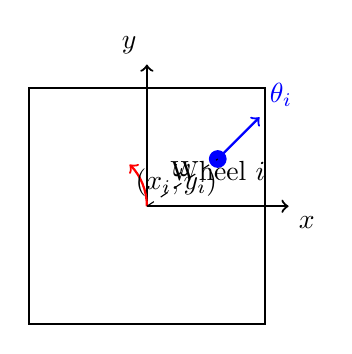
\begin{tikzpicture}[scale=1.5]
% Robot body
\draw[thick] (-1,-1) rectangle (1,1);
\draw[->, thick] (0,0) -- (1.2,0) node[anchor=north west] {\(x\)};
\draw[->, thick] (0,0) -- (0,1.2) node[anchor=south east] {\(y\)};
\draw[->, thick, red] (0,0) arc (0:45:0.5);
\node at (0.3,0.3) {\(\omega\)};

% Wheel
\filldraw[blue] (0.6,0.4) circle (2pt);
\draw[->, blue, thick] (0.6,0.4) -- +(45:0.5) node[anchor=south west] {\(\theta_i\)};
\node at (0.6,0.3) {Wheel \(i\)};
\draw[dashed] (0,0) -- (0.6,0.4);
\node at (0.25,0.2) {\((x_i, y_i)\)};
\end{tikzpicture}
\end{center}

\section{Conclusion}

The row vector \( \mathbf{h}_i \) provides a compact and elegant way to project full robot motion into the directional motion of individual wheels. This mapping is critical for control of omni-directional or mecanum drive systems in robotics.

\end{document}
